\documentclass[12pt]{article}
\usepackage{amsmath, amsthm, amssymb, pdfpages} 
\usepackage{fullpage}
\usepackage{hyperref}
\usepackage{graphicx}
\usepackage[capitalize]{cleveref}

\title{Testing the effectiveness of principal components in adjusting for relatedness in genetic association studies}
\author{Yiqi Yao, Alejandro Ochoa}

% To set proper spacing
\renewcommand{\baselinestretch}{1.2}

\begin{document}
\maketitle
	
\section{Introduction} 

The goal of a genome-wide association study (GWAS) is to identify loci whose genotypes are correlated significantly with a certain trait.
An important assumption made by basic association tests is that genotypes at non-associated loci are drawn independently from a common allele frequency, so that they are in Hardy-Weinberg Equilibrium (HWE).
However, HWE does not hold for structured populations, which includes multiethnic cohorts and admixed individuals.
When approaches for association not designed for structured populations are incorrectly applied to structured populations, association statistics (such as $\chi^2$) become inflated relative to the null expectation, resulting in greater numbers of false positives than expected.

Modern approaches for conducting genetic association studies with structured populations involve modeling the population structure via covariates.
Such covariates may be inferred ancestry proportions or transformations of these.
Principal components analysis (PCA) represents the most common of these variants, in which the top eigenvectors of the kinship matrix are used to model the population structure.
These top eigenvectors are commonly referred to as Principal Components (PCs) in the genetics literature (the convention we adopt here), but it is worth noting that in other fields the PCs would instead denote the projections of the data onto the eigenvectors.
Various works have found that PCs map to ancestry, and in GWAS work as well as ancestry but without the computational expense of inferring ancestry proportions.

The other dominant approach for genetic association studies under population structure is the Linear Mixed-effect Model (LMM), in which population structure is a random effect drawn from a covariance model parametrized by the kinship matrix.
LMM and PCA share deep connections that suggest that both models ought to perform similarly.
However, many previous studies have found that LMM outperforms the PCA approach, although many evaluations are inconclusive or are limited in the kinds of population structures they study, the magnitude of their differentiation, and other aspects of study design.
Moreover, various explanations for why LMM outperforms PCA are vague and have not been tested directly.
Since LMMs tend to be considerably slower than the PCA approach, it is important to understand when the difference in performance between these two approaches is outweighed by their difference in runtime.

In this work, we study the performance of the PCA method for GWAS, comparing it to a leading LMM approach, characterizing its behavior under various numbers of PCs and varying sample sizes, under a reasonable admixture model and a model with admixture and family structure.
We find that the performance of the PCA approach is favorable when sample sizes are large (at least 1,000 individuals), matching the performance of LMMs as long as enough PCs are used.
Remarkably, the approach is robust even when the number of PCs far exceeds the optimal number, suggesting that the degrees of freedom is not a concern in reasonably large studies.
However, for smaller studies (100 individuals) there is a more pronounced loss of power when the number of PCs exceeds the optimal number.
Moreover, PCA fails to perform as well as LMM in the presence of family structure, which is a scenario where the problematic structure is not low-dimensional so PCA naturally cannot model it entirely.
All together, our simulation studies provide clear criteria under which use of PCA results in acceptable performance compared to LMMs.

Missing:
\begin{itemize}
\item Proposed simulation to infer optimal number of PCs from real data, predict gap between PCA and LMM?
\item ...
\end{itemize}

\section{Methods}

\subsection{The additive quantitative trait model and PCA approximation}

Suppose there are $n$ individuals and $m$ loci,
$\mathbf{X}$ is their $n \times m$ genotype matrix, and
$\mathbf{y}$ is the length-$n$ (column) vector which represents trait value for each individual.
The PCA approach can be derived from the following additive linear model for a quantitative (continuous) trait:
$$
\mathbf{y}
=
\mathbf{1} \alpha + \mathbf{X} \mathbf{\beta} + \mathbf{\epsilon}
,
$$
where
$\mathbf{1}$ is a length-$n$ vector of ones,
$\alpha$ is the scalar intercept coefficient,
$\mathbf{\beta}$ is the length-$m$ vector of locus effect sizes, and
$\mathbf{\epsilon}$ is a length-$n$ vector of residuals.
The residuals are assumed to follow a normal distribution: $\mathbf{\epsilon} \sim \text{Normal}(0, \sigma^2)$, for some residual variance parameter $\sigma^2$.

Typically the number of loci $m$ is in the order of millions while the number of individuals $n$ is in the thousands.
Hence, the full model above cannot be fit in this typical $n \ll m$ case, as there are only $n$ datapoints to fit (the trait vector) but there are $m+1$ parameters to fit ($\alpha$ and the $\mathbf{\beta}$ vector).
The PCA model with $p$ PCs corresponds to the following approximation to the full model, corresponding to a model fit at a single locus $i$:
$$
\mathbf{y}
=
\mathbf{1} \alpha + \mathbf{x}_i \beta_i + \mathbf{U}_p \mathbf{\gamma}_p + \mathbf{\epsilon}
,
$$
where $\mathbf{x}_i$ is the length-$n$ vector of genotypes at locus $i$ only,
$\beta_i$ is the effect size coefficient for that locus,
$\mathbf{U}_p$ is an $n \times p$ matrix of PCs, and
$\mathbf{\gamma}_p$ is the length-$p$ vector of coefficients for the PCs.
This approximation is explained by first noticing that the genotype matrix has the following singular value decomposition:
$\mathbf{X} = \mathbf{U} \mathbf{D} \mathbf{V}^\intercal$,
where
$\mathbf{U}$ are its left singular vectors of $\mathbf{X}$,
$\mathbf{V}$ are its right singular vectors, and
$\mathbf{D}$ is a diagonal matrix of its singular values.
Thus, in the full model we have
$\mathbf{X} \mathbf{\beta} = \mathbf{U} \mathbf{\gamma}$,
where
$\mathbf{\gamma} = \mathbf{D} \mathbf{V}^\intercal \mathbf{\beta}$.
The approximation consists solely of replacing $\mathbf{U} \mathbf{\gamma}$ (the full set of $n$ left singular vectors and their coefficients) with $\mathbf{U}_p \mathbf{\gamma}_p$ (the top $p$ singular vectors only, which constitutes the best approximation of rank $p$).
Thus, the extra terms in the PCA approach approximate the polygenic effect of the whole genome, and assumes that the locus $i$ being tested does not contribute greatly to this signal.
An equivalent model can be arrived at after standardizing each locus of the genotype matrix, in which case $\mathbf{U}$ is also equal to the eigenvectors of the kinship matrix.

Statistical significance is tested as follows.
The null hypothesis is $\beta_j = 0$ (no association).
The null and alternative models are each fit (fitting the coefficients of the multiple regression, where $\beta_j$ is excluded under the null while it is fit under the alternative).
The resulting regression residuals are compared to each other using the F-test, which results in a p-value where here a two-tailed test is used.
Note that many common PCA implementations trade the more exact F-test for a $\chi^2$ test, which is simpler to implement but only asymptotically accurate.
As this is a multiple hypothesis test, there are a large number of loci ($m$) tested for association, so it is best to control the FDR rather than setting a fixed p-value threshold.
We recommend estimating q-values and setting a threshold of $q < 0.05$ so that the FDR is controlled at the 5\% level.

\subsection{Admixture Simulation}
The construction of admixture population is mainly based on admixture simulation of Alex (2016). The related code of admixture simulation has been uploaded to Github with a R package called "bnpsd".  Some parameters are changed in order to better simulate under different situation. According to Alex (2016), the number of independent loci is 30000, in this paper the number of independent locus is 10000. The default value of Alex (2016) is 3, whereas in this project, it can be variable. Considering the difference among number of sub-population, the sample size of $i_{th}$ sub-population will be set as the smaller integer of the ratio of total sample divided by number of sub-population.\\
Regarding the family structure, the generation will be set to be 20 to simulate admixture population with the existence of family structure. Considering the large calculation cost during the generation process of admixture population with family structure, this data set will be treated as real data set. It will be used repeatedly to test performance of PCA under different situations with random traits.



\subsection{Trait Simulation}
The construction of trait simulation is based on a R package called "simtrait". This package constructs the complex trait simulation with user-defined causal loci and the desirable heritability of the trait. It can be used in both simulated data set and real data set if the kinship matrix is estimated correctly. \\
In our simulation,the function of trait can be written as $$y=G+ \epsilon$$ 
, where G represents the effect of genotype and $\epsilon$ represents the noise. The noise follows a normal distribution with mean zero and variacne equals to one minus hertability rate times desired parametric variance factor of the trait which is 1 in default. To obtain the genotype effect, marginal allele frequency will be calculated first and then, SNP will be randomly selected as causal index with random SNP coefficients. Then  coefficients of causal index will be scaled and centered to estimate the genotype effect, thereby obtaining the numerical value of traits of each causal loci.The rank of genotype effect equals to the number of true subpopulation minus one as we take intercept into consideration as well.  


\subsection{Result Examination Method}

In this paper, precision-recall curves and uniformity p-value test will be used to test the performance of PCA under different scenarios. Both two methods will be illustrated by boxplot.

\subsubsection{Precision-Recall Curves}

Precision-recall curve is a plot whose y-axis represents precision and x-axis represents recall. Precision is calculated as the number of true positives divided by sum of both true positives which indicates the performance of model in predicting positives. Similarly, recall measures the ratio of number of true negatives and sum of true negatives and false negatives, which measures the performance of model in predicting negatives.Hence, the precision measures the relevancy of result which indicates the proportion of selected items are relevant. The recall shows the proportion of relevant items are selected. The precision and recall curve demonstrates the trade-off among precision and recall. Hence, the formula of precision and recall can be written as:
$$Precision=\frac{TP}{TP + FP}$$
$$Recall=\frac{TP}{TP + FN}$$

The area under the curve (AUC) is calculated as the integration of curve of precision and recall. It measures the aggregated performance of through different thresholds. The range of AUC is from 1 to 0. When AUC equals to 1, it can be interpreted as the predictions of model is $100\%$ correct, whereas, AUC equals to 0 indicates that all predictions of this model are wrong. 
\subsubsection{Uniform P-Value Test }
Due to the existence of multiply hypothesis test in our simulation, the frequency of erroneous inferences will increase. Altough Bonferroni Correction can be used to deal with this problem, it can result in high false negative rate (FNR). The better strategy is to controlling the False Discovery Rate (FDR). FDR is calculated as the ratio of flase positives and the sum of true positives and false positives.For multiple independent and identical hypothesis tests, if the null hypothesis is true, the distribution of p-values will approximate to a uniform distribution [8]. In this case, a bette strategy is to use the q-value rather than p-value to control the FDR. Therefore, we should evaluate the performance of PCA by quantifying the distribution of p-value of null hypothesis. If distribution of p-vlaues of null hypothesis is significantly deviates from the quantiles of uniform distribution, the resulting q-values are anti-conservative.Thus, we use root mean square deviation (RMSD) to measure the fittness of quantiles p-values to the expected quantiles of uniform distribution. The RMSD is calculated as the root mean square difference among sorted p-values of null hypothesis and expected quantiles of sorted p-values of null hypothesis after removing causal indexes.The numerical values of RMSD is inversely  performance of PCA. The formula of RMSD is:
$$
\text{RMSD}
=
\sqrt{ \frac{1}{m_0} \sum_{i = 1}^{m_0} \left( u_i - p_{(i)} \right)^2 },
$$
where
$m_0$ is the number of null loci (truly not trait-associated),
here $i$ indexes null loci only,
$p_{(i)}$ is the $i$th ordered null p-value, and
$u_i$ is its expectation (the $i/m_0$ percentile of the uniform distribution).

In previous evaluations, genomic control has been used to measure test statistic inflation, which results in non-uniform p-values.
The inflation factor $\lambda$ is defined as the median $\chi^2$ association statistic divided by theoretical median under the null hypothesis.
Hence, $\lambda = 1$ indicates no inflation, equivalent to uniform p-values (RMSD $ = 0$ above).
On the other hand, $\lambda > 1$ (results in RMSD $ > 0$) corresponds to inflated statistics, which occurs when residual population structure is present;
for PCA, this occurs when not enough PCs were used.
Although $\lambda < 1$ is possible, it is not expected for genetic association studies, although that case also results in RMSD $ > 0$.
Note that $\lambda$ only use the median of the null distribution to measure the non-uniformity of p-values, whereas the RMSD makes use of the complete p-value distribution to make this assessment, which should be more powerful.

\subsection{Comparison among PCA and Existing Implementations }

Some current research argue that Linear Mixed Model (LMM) can outperform PCA in correcting for population strcuture. In Linear Mixed Model, population strcuture is treated as random effect. Gengxin and Hongjiang (2013) demonstrate that efficient
mixed-model association eXpedited (EMMAX) which is based on linear mixed model outperforms PCA in both the population cohort study and case-control study. In this project, LMM will be tested under the same admixture simulation and trait simulation to PCA and thus, comparison between LMM and PAC with different PCs used under different situations can be made. Additionally, PCA with no PC used is equivalent to Linear Regression (LM). We will also consider the performance comparision among PCA and LM. 



\section{Result}

We use simulation data where genotypes and trait will be simulated following procedure mentioned above. We first set the sample size to be 1000 and then, we reduce the sample size to 100 to investigate whether PCA still have similar performance under new scenario. We will conduct 10 times simulation so that the extra variance can be reduced. For each simulation, performance of PCA will be collected in terms of RMSD and AUC for PCs from 2 to 90. Also, real data set will also be introduced to test the performance of PCA and trait will be simulated in the same way to simulation data. Then, We will test the performance of PCA when family structure exists with sample size equals to 1000 and 100 separately. Finally, we test the performance of PCA with the existence of complex family structure and here we set the generation to be 20.

\subsection{PCA performance under N=1000}
\begin{figure}[bp!]
  \centering
  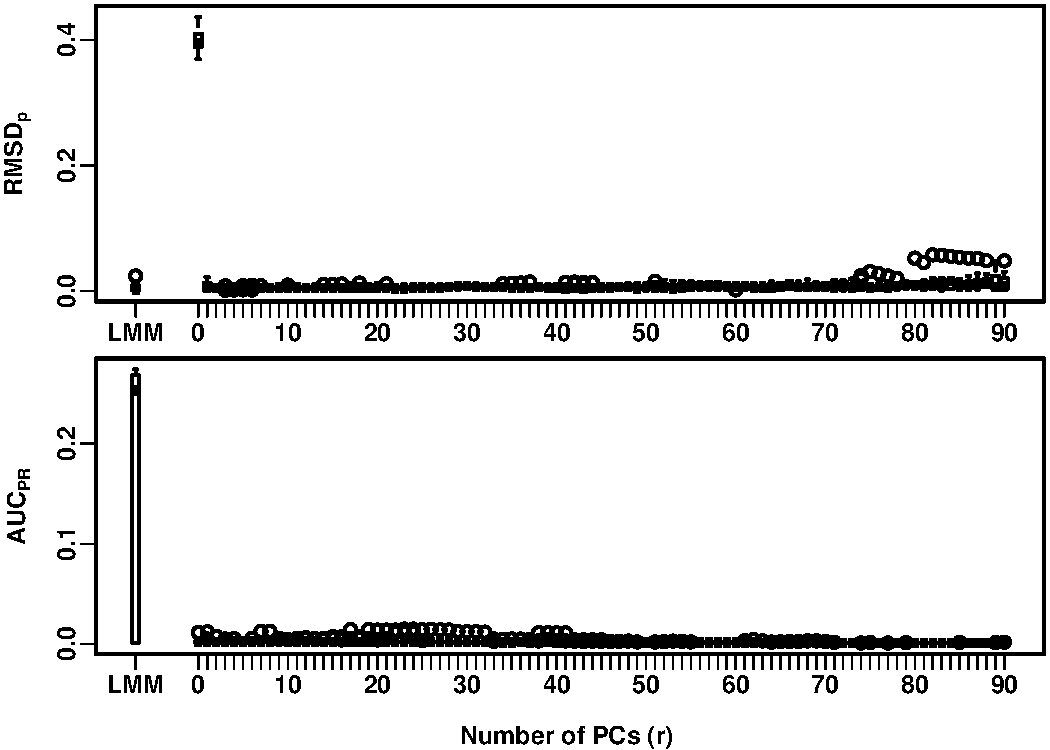
\includegraphics[width=4in]{PCA_n_1000_m_10_k_10.pdf}
  \caption{
    {\bf boxplot of rmsd and auc}
    The first panel is the boxplot of RMSD when sample size is 1000. Here the y axis represents value of rmsd and x axis is the number of PCs used in PCA.
    The second panel is the boxplot of AUC and here y axis is value of AUC. RMSD is used to measure the deviation of distribution of p values of null hypothesis from uniform distribution. In the case of multiple null hypothesis holds, the distribution of p-values of null hypothesis should approximate to unifrom distribution. The small value of RMSD implies type one error is well controlled. Regaring AUC, it's calculated by integration of predicion and recall curve. The value of AUC can be interpreted as the proportion of predictions made by this model is correct. The large AUC value implies better performance in predictive power. The result of Linear Regression is put at the position of PC equals to zero and the result of LMM is put at the position of PC equals to 91.}
  \label{fig:example}
\end{figure}

According to the first panel in Figure 1 which is the boxplot of RSMD when the number of subpopulation is 10 and sample size is 1000, it can be seen that RMSD values remain relatively high when p is smaller than 9, which satisfies the actual rank of genotype matrix or kinship matrix which is (k-1). It demonstrates that the distribution of p-values of null hypothesis deviates from the expected quantiles of uniform distribution and therefore, PCA fails to control FDR.Though the performance of PCA is relatively bad, there still exists an decreasing tendency. It indicates that when the number of PCs used in PCA is smaller than true rank of genotype matrix, PCA will benefit forom using more PCs in terms of controlling FDR. However, once the number of PCs used in PCA reaches the actual rank of genotype matrix or kinship matrix, the RSDM will junmp to a small value and in this case the value of RMSD is close to 0. It remains stable as the number of PCA increases. Apart from this, it can be seen that before the number of PCs reaches the rank of genotype matrix, the distance among minimum and maximun of RMSD is larger. It tends to be smaller after number of PCs used in PCA is larger than the rank of genotype matrix, which shows less fluctuations in terms of type 1 error controlling. The RMSD value of LM is around 0.13 and it is smaller than PCA's RMSD value when PCs used in PCA is smaller than true rank of genotype matrix. However, once the number of PCs is larger than true rank of genotype matrix, it can be seen that PCA has better performance in type one error controlling. Compared with the performance of LMM, it can be seen that both PCA and LMM controll type one error well once the number of PCs used in PCA is larger than the true rank of genotype.\\

The seond pandel of Figure 1 illustrates the pattern of AUC for the same scenario to the first panel. In this case, we can see a increasing tendency for AUC when the number of PCs is samller than the true rank of genotype or kinship matrix. Such a tendency indicates that the increase of number of PCs can increase predictive power of PCA when it is smaller than the rank of genotype matrix. Once the number of PCs used in PCA exceeds the rank of PCA, the value of AUC will be increased to around 0.8, which indicates that $80\%$ predictions of PCA are correct. After that, PCA does not benefit from adding more PCs as it can not increase the value of AUC obviously. Similarly, the range of AUC tends to be smaller than it when the number of PCs used in PCA is greater than rank of genotype matrix. It is clear that LM has better performance when  Similar to the previous pandel, PCA outperforms LM when the number of PCs is no smaller than the true rank of genotype matrix. In terms of LMM, the average AUC value is slightly higher than AUC of PCA even the number of PCs is larger than true rank of genotype matrix. \\


\subsection{PCA performance under N=100}
\begin{figure}[bp!]
  \centering
  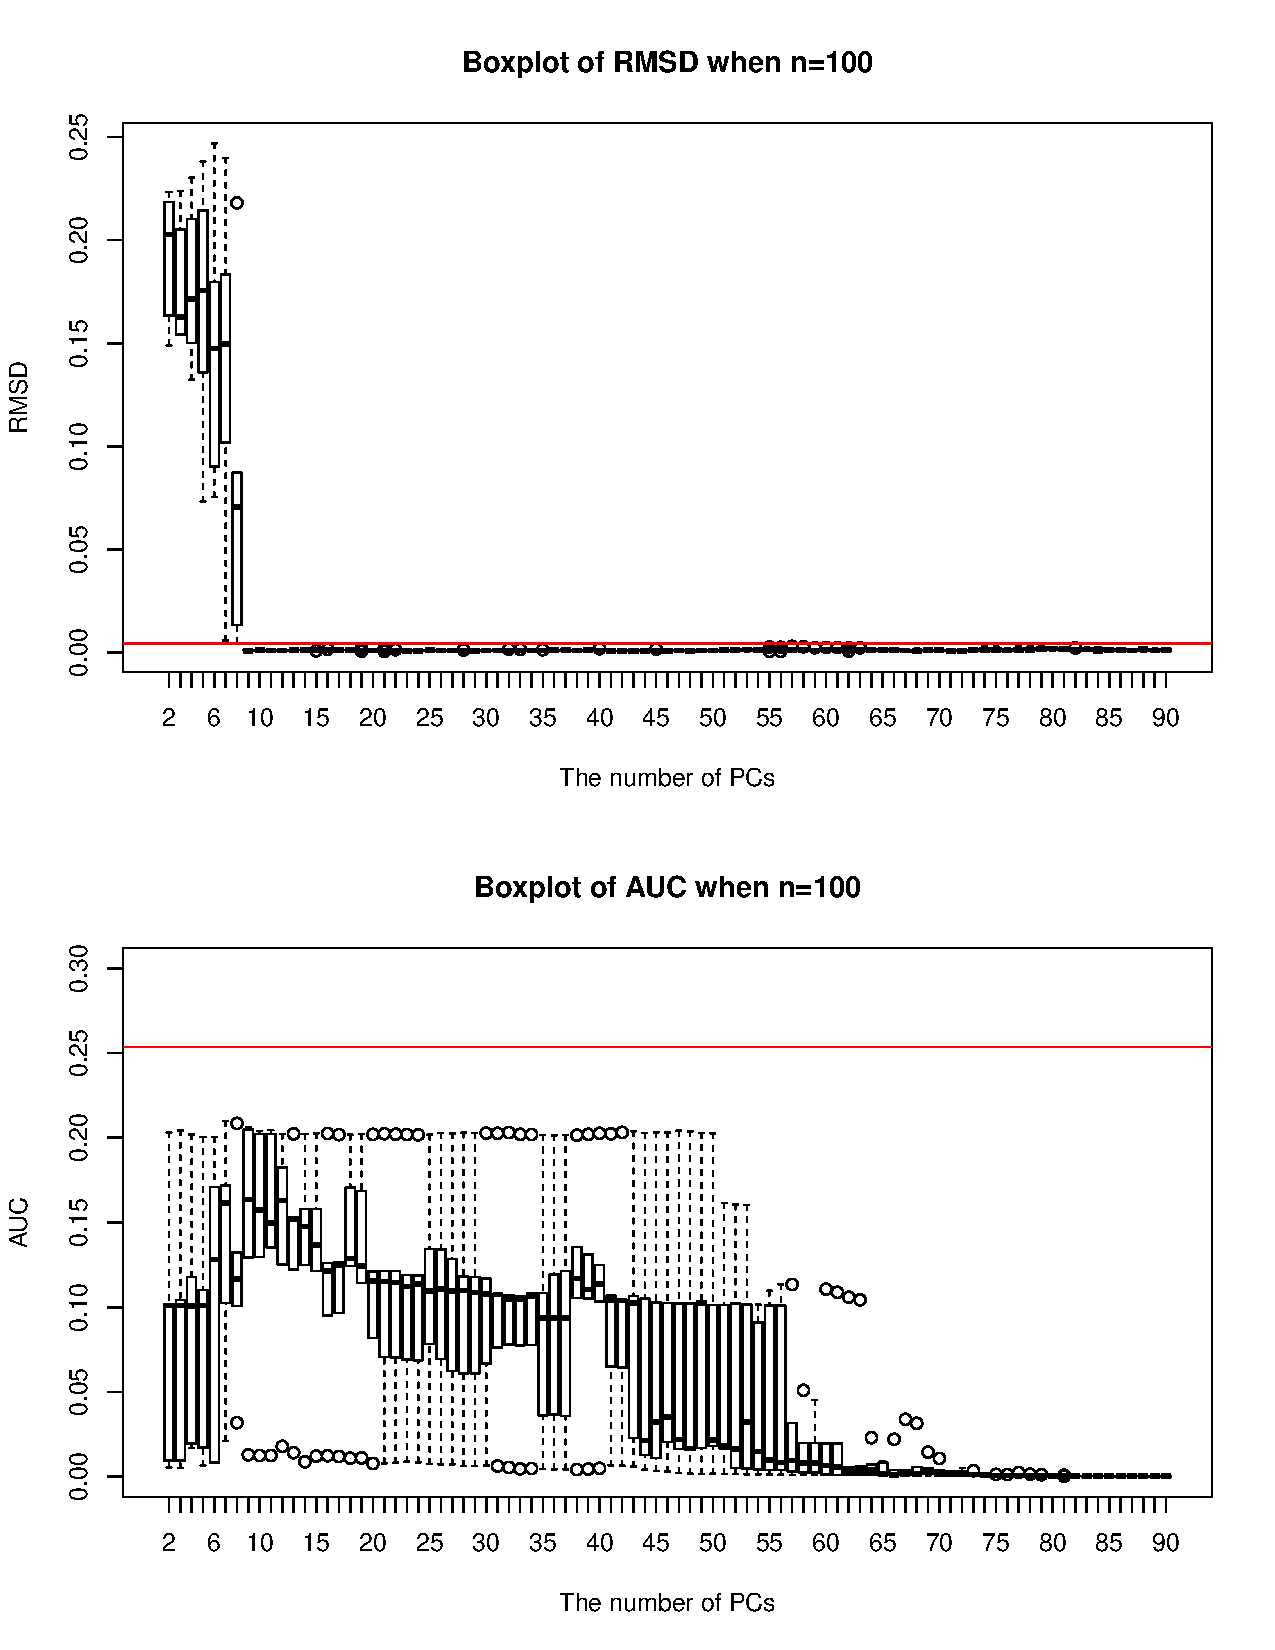
\includegraphics[width=4in]{PCA_n_100_m_10_k_10.pdf}
  \caption{
    {\bf boxplot of rmsd and auc}
   The first panel is the boxplot of RMSD when sample size is 100. The pattern of panel A in Figure 2 is similar to the first panel in Figure 1. The converging value of RMSD here is also close to zero indicating that even in a small sample size, PCA is still robust to type one error controlling. Moreover, the LMM and PCA has similar RSMD values which demonstrates that these two methods have almost the same performance in type one error controlling. The pattern of second panel in Figure 2 is bell-shapled. The AUC value reaches the peak when the number of PCs used in PCA equals to 9 and begins to decrease with the increase of PCs used. It illustrates that PCA fails in terms of power when the sample size is small. The decrease tendency is more obvious when the number of PCs is around 68 and it can be seen that LMM which is located at the last point of y-axis has better performance in power, compared with PCA and LM.  }
  \label{fig:example}
\end{figure}

Then, we want to investigate the performance of PCA when samlpe size is samll. Here we set the sample size to be 100. From the first panel of Figure 2, it can be seen that the pattern is similar to the boxplot of RMSD in the case of sample size equals to 1000. It illustrates an decreasing when the number of PCs is smaller than true rank of genotype matrix. It indicates that PCA can better control type 1 error in this situation. If the number of PCs is greater than true rank of genotype matrix, the RSMD will decrease immediately and approximate to zero, which shows type one error is excellently controlled. Hence, PCA is insensitive to the smaple size in terms of RMSD or type 1 error controlling. Campored with the RMSD value of LM, RMSD value of PCA is smaller when the number of PCs is greater than 3.It implies that PCA control type one error better than LM. Moreover,the performance of LMM in this case is similar to Figure 2 which is close to previous figure. The RMSD value of LMM approximates to 0 which indicates that there is no significant difference among PCA and LMM in this csae.\\

Concerned with the boxplot of AUC, the pattern is obviously different from the boxplot of AUC when smaple size is 1000. Although we still can find an increasing pattern of AUC before the number of PCs reaches the k. However, it can be seen that there is an decreasing pattern of AUC value once the number of PCs exceeds the true rank of PCA. It demonstrates that, even though fluctuations exist, performance of PCA in terms of power can be wrose with the increase of PCs used in PCA. The position of peak of AUC in this case is located at PCs equal to 9 which is exactly the true rank of genotype. Since we take the intercept into consideration, the true rank of genotype matrix equals to the number of subpopulation minus one. The bell-shaled distribution of AUC boxpolot implies that PCA receives punishment in power once the number of PCs used in PCA is larger than true rank of genotype matrix. Moreover, in terms of LM, it can be seen that even only one PC is used in PCA, the AUC value of PCA is still no worse than LM. However, when  excessive PCs are used, performance of LMM can be better with a larger AUC value. Considering LMM, the average` AUC value is 0.25, whereas, the maximum AUC of PCA is 0.2 and it decreases immediately due to the excessive use of PCs. In this case, LMM performs better than PCA in terms of power. \\




\begin{figure}[bp!]
  \centering
  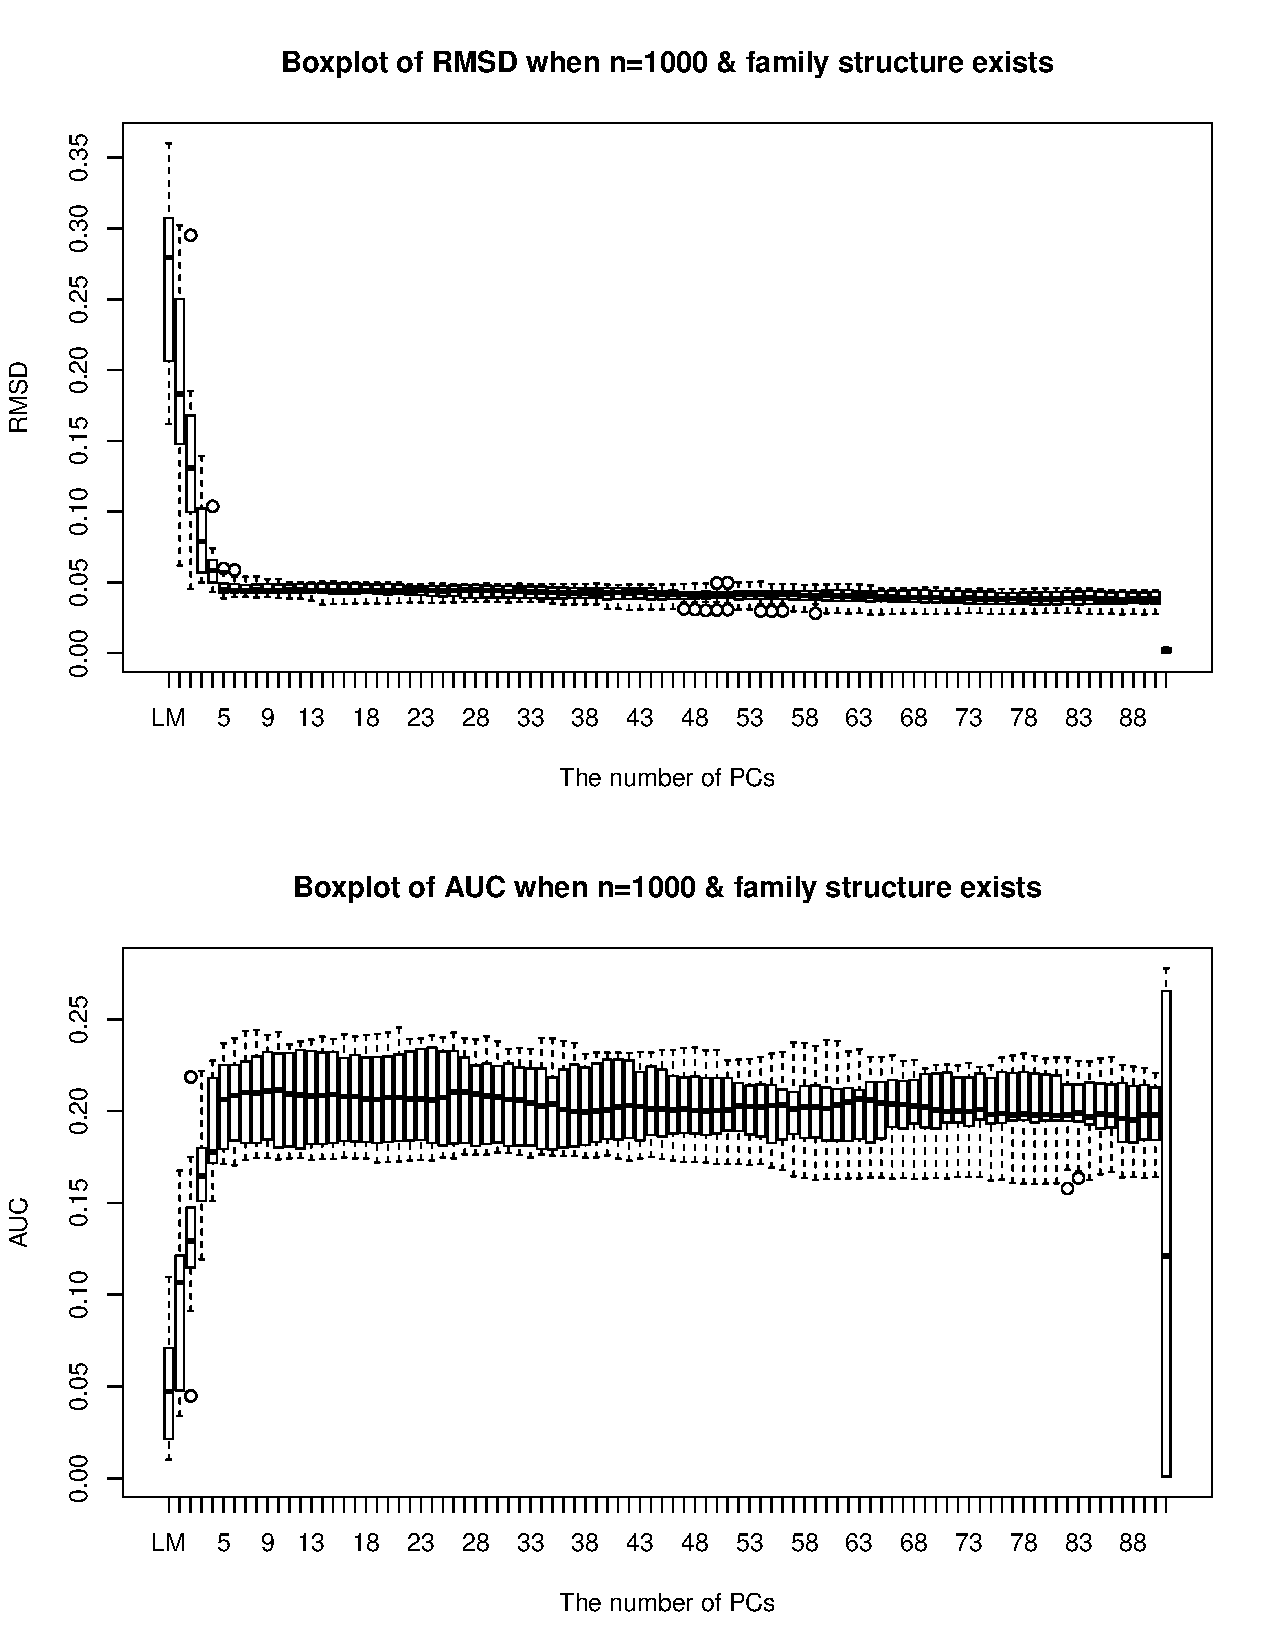
\includegraphics[width=4in]{PCA_n_1000_m_100_family_structure.pdf}
  \caption{
    {\bf boxplot of rmsd and auc}
    The first panel is the boxplot of RMSD when sample size is 100. The pattern of panel A in Figure 2 is similar to the first panel in Figure 1. The converging value of RMSD here is also close to one indicating that even in a small sample size, PCA is still robust to type one error controlling. The pattern of second panel in Figure 2 is bell-shapled. The AUC value reaches the peak when the number of PCs used in PCA equals to 9 and begins to decrease with the increase of PCs used. It illustrates that PCA fails in terms of power when the sample size is small. E}
  \label{fig:example}
\end{figure}

\subsubsection{PCA performance when familty structure exists}

The introduction of family structure will make the original admixture populatio more complicated. In this csae, we assume that there are 20 generations in total while other factors fixed. Based on the result of the first panel in figure 3 indicates that there is a decreasing pattern of RMSD for the first three PCs. It addition, the value of RMSD in this situation is large, which indicates that the distribution of p-value of null hypothesis does not approximate to uniform distribution. It illustrates that PCA fails to control type one error when the number of PCs is not enough. When the number of PCs is larger than 4, values of RMSD beome stable around 0.05 which demonstrates that there exists evidence of the distribution of p-value of null hypothesis does not deviate from uniform distribution but the evidence is weaker than previous simulation where RSDM approximates to 0. Considering the range of RMSD, it decreases first and then begins to increase. It shows that excessive use of PCs will lead to extra variance.For AUC, it illustrates an increasing tendency for the first three PCs. When the number of PCs is larger than 3, AUC fluctuates around 0.2. This shows the power of PCA is small and hence, PCA's performance is not pretty well in this csae in terms of power even though enough PCs are used. 


\section{Discussion}
\subsection{PCA GWAS fails without enough PCs}
Right now, both LMM and PCA have become standard approaches to correct for admixture population. In current PCA GWAS research, the number of PCs used in PCA is ususally assmued to be 10. For instance, based on the simulation of Hoffman (2013), 10 PCs are randomly selected from the first 30 PCs. Furthermore, Genevieve et al. (2019) also performed PCA GWAS for 26 traits with first 10 PCs. According to the result of Genevieve et al. (2019), the correlation plot between SNP genotype and PC1–PC10 illustrates different populations has different correlations over some PCs. It seems that there exists a tradition that when PCA GWAS is performed, the top 10 PCs will be used. Since the result of PCA GWAS in this convention is good, right now most paprs will assume the number of PCs used in PCA GWAS to be 10. However, in this paper, we further investigate about the optimal choice of number of PCA under different population structures. In most current research, the number of subpopulation is smaller 10 and thus, based on results of previous three scenarios, the number of PCs used in PCA is enough which certifies the good performance of PCA  in current research. For instance, based on the scatter plot of first two principal components with HapMap3 dataset which contains 11 populations, it can be divided into three subpopulations (Gad and Machiel, 2014). On the contraty, the lack of PCs will lead to the failure of PCA regardless of the sample size or family structure in both type one error and power. Seokho et al.(2012) state that considering the large number of single-nucleotide polymorphisms (SNP) used in GWAS to infer structure, it is necessary to remove SNPs that have negligible loadings in PCA. Whereas, our simulation indicates that if there is no enough PCs used in PCA GWAS, its performance can be bad as SNPs that have significant loadings are vanished from the analysis.


\subsection{PCA GWAS still works even too many PCs are used}
PCA GWAS is still robust even though PCs are excessively used for type one error controlling. However, for power, it will receive punishment if the number of PCs are excessive and the sample size is small. Jason and Anna (2009) point out that PCA with large sample size has better sample size than it with small sample size. This is because that PCA with large sample size can have smaller probability error and larger accuracy of population estimation ( Jason and Anna ,2009). The small sample size in our research project only has 100 individuals in total. In a GWAS study, this is an extreme situation which it not realistic in research. The AUC boxplot of small sample size indicates that the peak of AUC is close to AUC value for large sample size. This may result from that the number of causal loci in small sample size is reduced from 100 to 10.However, the boxplot of AUC has a bell shap with downward-sloping line on each side of the peak. It demonstrates that in small sample size, punishment of excessive use of PCs will come occur immdeiately. Considering in the study of GWAS, we will expect to use thousnds of SNPs and number of individuals are also much larger than 100, the situation of small sample size may not be common (Seokho et al., 2012). Hence, although PCA will fail when the number of PCs is much larger than the true rank of genotype matrix, it is still encouraged to use more PCs in PCA GWAS .

\subsection{PCA GWAS fails with the existence are close relatives }
Alkes et al.(2010) point out that GWAS may fail in the case of dataset contains  family structure. The result of our simulation also supports this argument. Figure 3 shows that 
\subsection{LMM outperforms PCA }
Wang et al. (2013) argues that mixed effects model is preferred in the case of existence cryptic relatedness but not population stratification. In their paper, only first four PCs are used in PCA and performance of PCA may be underestimated. Fruthermore, EMMAX which is a kind of linear mixed model is claimed to be better than PCA (Gengxin and Hongjiang, 2013). Based on the result of our simulations, it can be seen that in both large sample size and small sample size, LMM are slightly better than PCA in terms of power. When sample size is large such as the scenario in figure 1 panel B, it can be seen that although both two methods's are not good. However, the maximum AUC value of PCA is around 0.25 and LMM's AUC value is slightly larger than PCA. In addition to this, in the case of small smaple size, advantage of LMM is more obvious. As mentioned before, PCA will receive punishment when the number of PCs is much larger than the true rank of genotype matrix. The maximum of AUC value of PCA in this scenario decreases to 0.2 and the average AUC value of LMM is around 0.24. This two simulations illustrates that 



\end{document}
